\documentclass[a4paper]{article}

\usepackage[dvipsnames,usenames,svgnames,table]{xcolor}
\usepackage{amsmath}
\usepackage{amssymb}
\usepackage[english]{babel}
\usepackage{caption}
\usepackage{csquotes}
\usepackage{empheq}
\usepackage{enumitem}
\usepackage{float}
\usepackage[bottom]{footmisc}
\usepackage{geometry}
\usepackage{graphicx}
\usepackage{hyperref}
\usepackage{cleveref}
% NOTE: the ordering is important!
\usepackage[toc]{glossaries}
\usepackage[utf8]{inputenc}
\usepackage{multicol}
\usepackage{multirow}
\usepackage{tikz}
\usepackage{titleps}
\usepackage[nottoc,numbib]{tocbibind}
\usepackage{trfsigns}
\usepackage{url}
\usepackage{wrapfig}

% Setup of pagestyle
\newpagestyle{fancypage}{
  \headrule
  \sethead{\MakeUppercase{\sectiontitle}}{}{\subsectiontitle}
  \setfoot{}{\thepage}{}
}
\settitlemarks{section,subsection,subsubsection}
\pagestyle{fancypage}

% Setup links
\hypersetup{
    linktoc=all,
    citecolor=gray,
    linkcolor=magenta,
    colorlinks=true,
}

\geometry{
 landscape,
 left=15mm,
 right=15mm,
 top=20mm,
 bottom=20mm,
}

\newcommand*\widefbox[1]{\fbox{\hspace{1em}#1\hspace{1em}}}
\newcommand{\circlesign}[1]{
    \mathbin{
        \mathchoice
        {\buildcirclesign{\displaystyle}{#1}}
        {\buildcirclesign{\textstyle}{#1}}
        {\buildcirclesign{\scriptstyle}{#1}}
        {\buildcirclesign{\scriptscriptstyle}{#1}}
    }
}
\newcommand\buildcirclesign[2]{%
    \begin{tikzpicture}[baseline=(X.base), inner sep=0, outer sep=0]
    \node[draw,circle] (X)  {\ensuremath{#1 #2}};
    \end{tikzpicture}%
}
\DeclareMathOperator{\sinc}{sinc}
\DeclareMathOperator{\SNR}{SNR}
\DeclareMathOperator{\Var}{Var}

\graphicspath{ {img/} }

\setlength\columnseprule{0.5pt}
\setlength{\columnsep}{10mm}
\setlength{\parindent}{0mm}
\setlength{\abovecaptionskip}{5pt}
\setlist[1]{itemsep=-0.1em}

\title{\vspace*{\fill}Summary of Cloud Computing at University of Bristol 2018 / 2019\footnote{This is just a simple summary.
I am not responsible for the provided content or anything which belongs to this. If there are any questions please contact me at
bauerflorian13@gmail.com .}}
\author{Florian Bauer\vspace*{\fill}}

\setcounter{secnumdepth}{0}

\begin{document}
  \begin{titlepage}
    \clearpage
    \maketitle
    \thispagestyle{empty}
  \end{titlepage}

  \begingroup
    \hypersetup{linkcolor=black}
    \clearpage
    \tableofcontents
    \thispagestyle{empty}
  \endgroup
  \pagebreak

  \setcounter{section}{-1}
  \setcounter{page}{1}
  \begin{multicols}{3}

\section{Lecture 01: Introduction}

\subsection{Comparison of the internet and electricity network}
\begin{itemize}
    \item starts with everyone has his own (electricity/ computationally power)
    \item connection between every single users grows
    \item ends in an all connected world with only a few big services provided by a small number of providers
    (computationally power goes from the device of the endusers to the cloud, electricity comes from big providers) 
\end{itemize}

\subsection{Normal Failure}
\begin{itemize}
    \item cloud data centre with $99.999\%$ survival rate
    \item $500 000$ server, probability of $100\%$ of the servers are still running after 3 years is $1\%$.
    \item \textbf{solution}: modular data centres, \textit{servers in container boxes}
\end{itemize}

\subsection{Essential Characteristics of Cloud Computing}
This definition belongs to NIST's characteristics of Cloud Computing
\begin{itemize}
    \item \textbf{On-demand self service}
    \item \textbf{Broad network access}
    \item \textbf{Ressource pooling}
    \item \textbf{Rapid elasticity}
    \item \textbf{Measured service}
\end{itemize}

\subsection{A common stratification: *aaS}
\label{subsec:everythingasaservice}
Everything as a Service.
\begin{itemize}
    \item \textbf{SaaS}: \textit{Software as a Service}, for instance: everyone
    \item \textbf{PaaS}: \textit{Platform as a Service}, for instance: \textit{Google App Engine}, \textit{Amazon Appstream}
    \item \textbf{IaaS}: \textit{Infrastructure as a Service}, for instance: \textit{Amazon EC2, S3}, \textit{Google Compute Engine}
\end{itemize}

A small number of companies providing IaaS/PaaS s services. Convergence to an oligopoly of less than five providers seems certain.

\section{Lecture 02: Coursework}

Just a few informations about the coursework and programming project. May be hopefully not important for the exam...

\section{L03: Economics of Cloud}

\subsection{The basic Economics}
\begin{itemize}
    \item \textbf{Cap}ital \textbf{Ex}penditure: \textit{Capex}
    \item \textbf{Op}erating \textbf{Ex}panditure: \textit{Opex}
    \item Capex vs Opex: \textit{Why buy a cow if all you need is the milk?}
\end{itemize}

\subsection{A typical warehouse scale computer}
\begin{itemize}
    \item \textit{pizzabox} in a \textit{refrigerator} is a server rack
    \item multiple server racks together are a cluster
    \item see \Cref{fig:warehousescalecomputer}
\end{itemize}

\begin{figure}[H]
    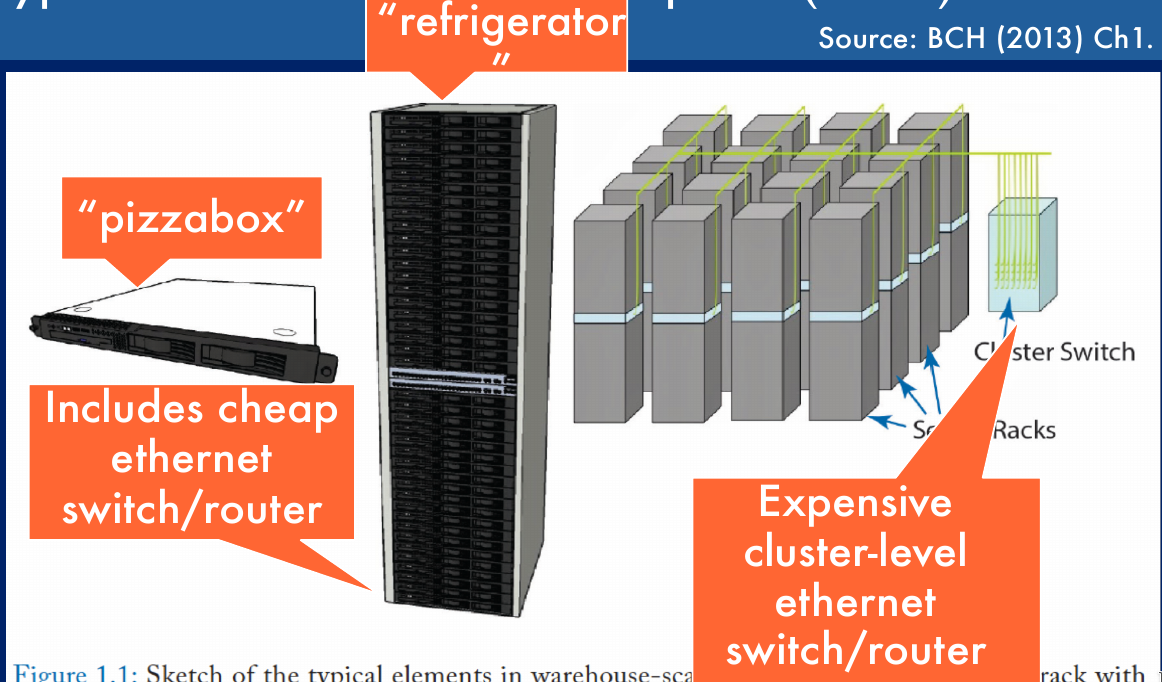
\includegraphics[width=\linewidth]{warehousescalecomputer.png}
    \caption{WSC - Warehouse-scale Computer}
    \label{fig:warehousescalecomputer}
\end{figure}

\subsection{Energy \& Power Efficiency}
\begin{itemize}
    \item cooling cost are around $42\%$
    \item optimizing the cooling efficiency will lower the overall costs massivley
\end{itemize}

\subsection{Resume}
\begin{itemize}
    \item there is a lot going on \textit{under the hood of a WSC} (WSC = \textbf{Warehouse-scale Computer})
    \item \textit{prod$>>$dev}: The innovations are made by and in companies not universitys
\end{itemize}

\section{L05: *aaS}
Definiton see in the Introduction section (Everything as a Service).%\cref{subsec:everythingasaservice}

\subsection{Why Xaas or *aaS}
\begin{itemize}
    \item avoiding of \textbf{Undiffertiated Heavy Lifting}
    \item the cloud is an ideal environment providing \textit{scale}, \textit{low cost}, \textit{automation via Infrastructure-as-Code}
\end{itemize}

\begin{figure}[H]
    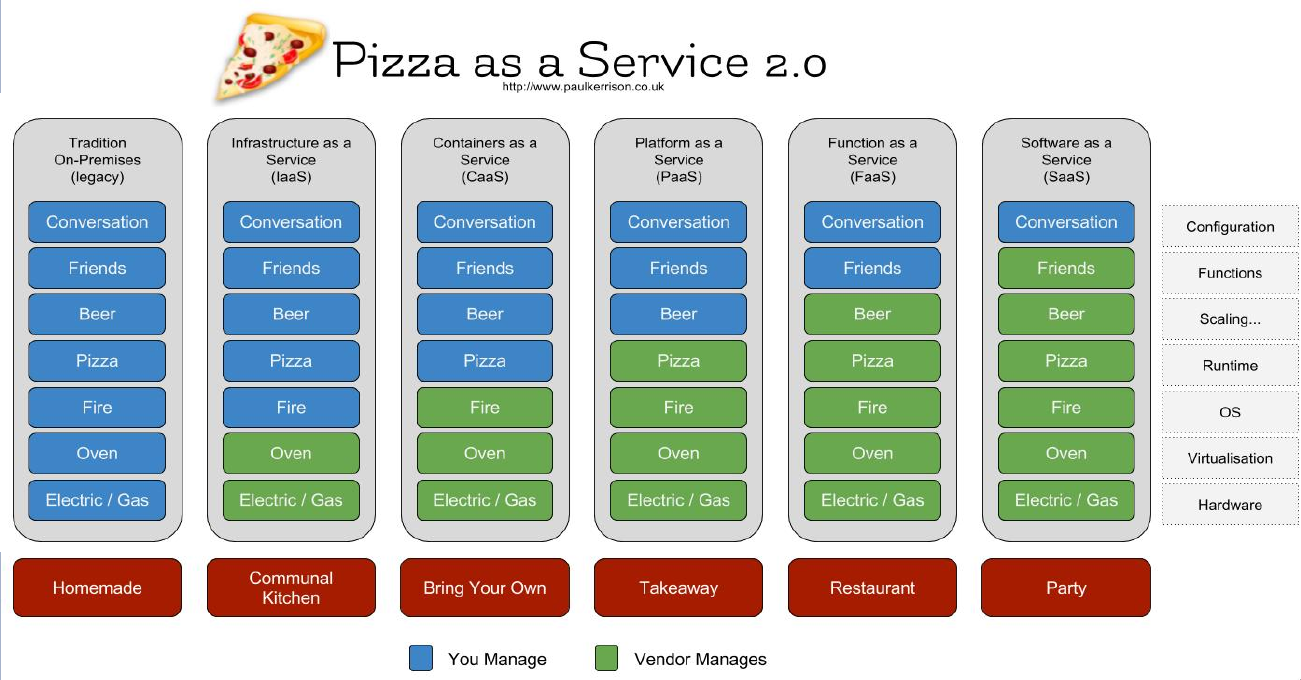
\includegraphics[width=\linewidth]{pizzaserviceexample.png}
    \caption{Pizza as a Service Example for *aaS}
    \label{fig:pizzaservice}
\end{figure}

\subsection{Structure of AWS Cloud}
\begin{itemize}
    \item \textbf{Availability Zones}: cluster of independent data centres, enables \textbf{fault isolation} and \textbf{high availability}
    \item \textbf{Regions}: entirely independent clouds, consists of a least two \textit{AZ}s, interconnection on global backbone, different regions have different costings
\end{itemize}

\subsection{Which Region should I choose?}
\begin{itemize}
    \item \textbf{Data souvereignty and compilance}: where to store user data?
    \item \textbf{Proximity of users to data}: where are the most of my users? -> lowest latency
    \item \textbf{Services and feature availability}: services and features may vary
    \item \textbf{Cost effectiveness}: each region has different costs (Europe and US are the cheapest)
\end{itemize}

\subsection{High Availability \& Fault Tolerance}
\textbf{High Availability:}
\begin{itemize}
    \item minimise service downtime by using redundant components
    \item require components in at least two AZs
    \item IaaS may have HA, PaaS usually will have HA
\end{itemize}

\textbf{Fault Tolerance}
\begin{itemize}
    \item ensure no service disruption by using active-active architecture
    \item requires service components in at least three AZs
    \item Iaas is unlikely to offer FT, PaaS some offers FT
\end{itemize}

\subsection{AWS Storage options}
\begin{itemize}
    \item Elastic Block Storage: SSDs, Magnetic, NAS, Use: OS, Apps
    \item S3: durable object storage, very cheap and big
    \item Instance Storage: on-host storage, very fast, caching
    \item Elastic File Store: shared storage across AZs
\end{itemize}

\subsection{IaaS vs PaaS}
\begin{itemize}
    \item IaaS mainly used by SysAdmins, PaaS mainly used by Developers
    \item IaaS provides e.g. \textit{VMs},\textit{Storage Services},\textit{Networking}, PaaS provides e.g. hosted databases, \textit{App deployment and managment env.},\textit{test suites}
    \item IaaS lower cloud costs, PaaS lower human costs
\end{itemize}

\section{L07: Virtualisation, Containers and Container Orchestration}

\subsection{Virtualisation Basics}
\begin{itemize}
    \item server hardware should be hidden from the user, $\rightarrow$ user sees only guest OS in a VM and not the host OS
    \item Amazon offers different VMs (\textit{AMIs}) with Linux or Windows
    \item VMs are created and run by the \textit{Virtual Machine Monitor (VMM)} aka the \textbf{hypervisor}
    \item VMs can stopped, copied, paused and resumed, which enables \textbf{server consolidation}: compress VMs to freeup servers
\end{itemize}

\subsection{Types of Virtualisation}
 Have a look at \Cref{fig:vmtypes}

\begin{figure}[H]
    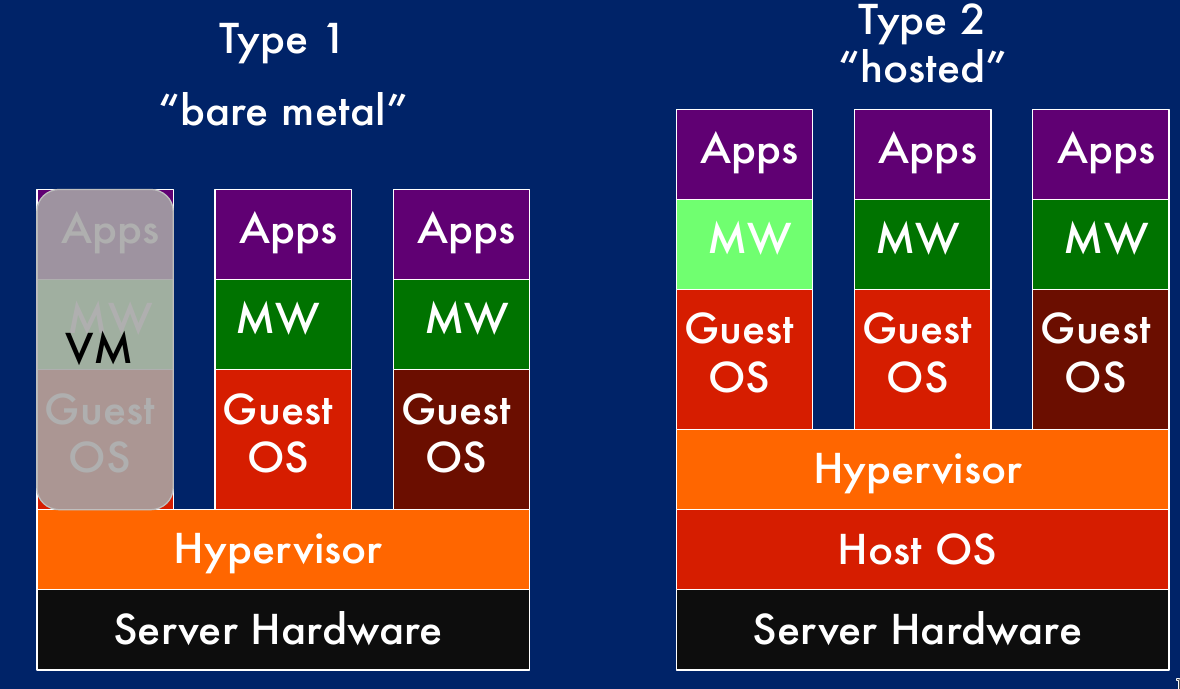
\includegraphics[width=\linewidth]{vmtypes.png}
    \caption{The two different virtualisation types}
    \label{fig:vmtypes}
\end{figure}

\textit{Xen} is an example for Type 1 VMs.

\begin{itemize}
    \item \textbf{Full virtualisation}: complete simulation of underlying guest machine hardware
    \item \textbf{Paravirtualisation}: guest OS can make Syscalls via the hypervisor's API, hypervisor does not simulate hardware
\end{itemize}

\subsection{Containerisation: Docker}
\begin{itemize}
    \item package and run application in lightweight, isolated environment
    \item Docker runs user processes in a super-isolated execution mode
    \item \textit{operating system level virtualisation} with shared kernel
    \item Advantage: No need to boot a whole VM
    \item Disadvantage: Potentially more insecure than complete virtualisation
\end{itemize}

\textbf{Docker Objects}
\begin{itemize}
    \item \textbf{Images}: read only template with instructions how to create a Docker Container
    \item \textbf{Container}: runnable instance of an  image, but ephemeral $\rightarrow$ all changes not mounted to persistend storage will be lost
\end{itemize}

\begin{figure}[H]
    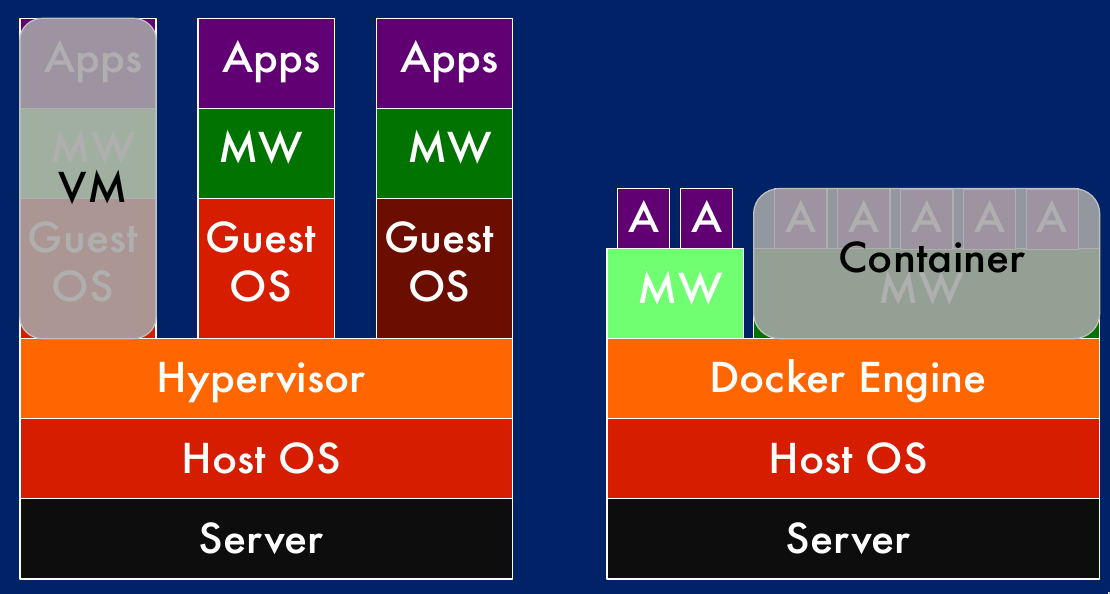
\includegraphics[width=\linewidth]{vmvsdocker.png}
    \caption{VMs vs Docker architecture schema}
    \label{fig:vmvsdocker}
\end{figure}

\subsection{Container Orchestration: Kubernetes}

\subsubsection{Motivation}
\begin{itemize}
    \item To run containers at scale needs managment tools
    \item \textbf{(Horizontal) Auto-scaling on demand}
    \item \textbf{Fault Tolerance}
    \item \textbf{Manage Accessibility from the web}
    \item \textbf{update/rollback without downtime}
\end{itemize}

\subsubsection{Featues of Kubernetes}
\begin{itemize}
    \item \textbf{Automated scaling}
    \item \textbf{Self healing}
    \item \textbf{Horizontal scaling}
    \item \textbf{Service discovery and Load Balancing}
    \item \textbf{Automated Rollbacks/Rollouts}
\end{itemize}

\subsubsection{Kubernetes Components}
\begin{figure}[H]
    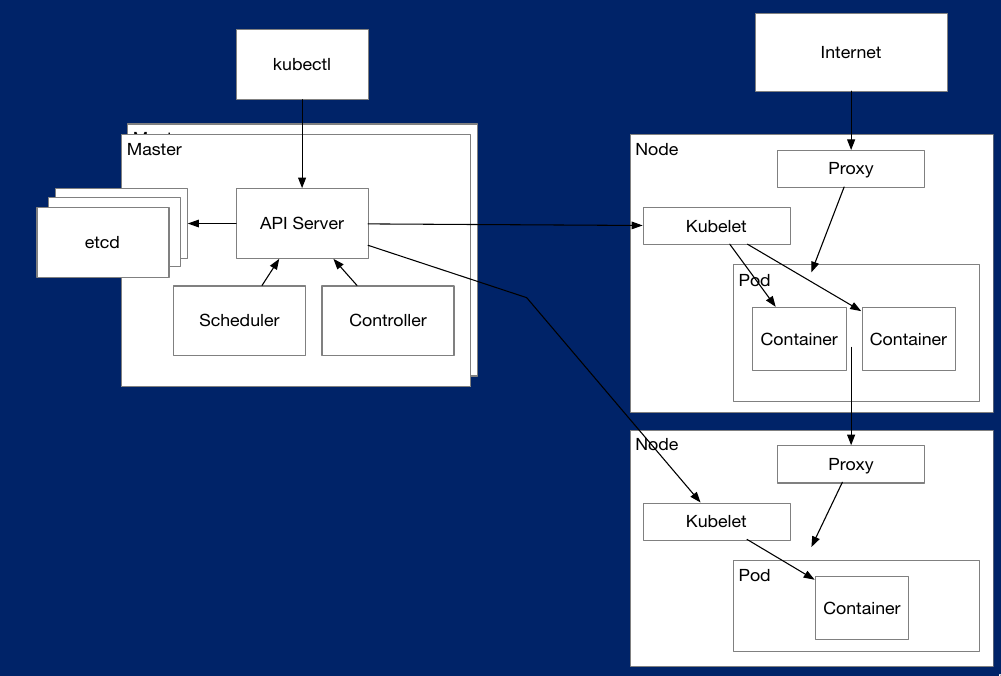
\includegraphics[width=\linewidth]{KubernetesComponents.png}
    \caption{Components of the Kubernetes architecture}
    \label{fig:kubernetescomponents}
\end{figure}

\begin{itemize}
    \item \textbf{Master}: manages the cluster state, subcomponents: \textbf{API Server}, \textbf{Controller}, \textbf{Scheduler}, writes to \textit{etcd} 
    \item \textbf{Nodes}: run work in pods, \textbf{Pods} are the scheduling unit, \textbf{Kubelet} is the agent to communicates with master, \textbf{Kube-proxy} is the network agent
    \item \textbf{Kubeclt}: local cli to controll cluster
    \item \textbf{Etcd}: distributed key-value store
    \item \textbf{Deployments}: \textbf{Replica Sets}, balances the number of running and scheduled pods; deployments provide update to Pods or ReplicaSets
    \item \textbf{Services}: groupings of pods which can be referred by a name, Unique IP and DNS name; Pods in Services are load balanced 
\end{itemize}

\section{L09: Serverless}

\textbf{Definiton}: \textit{The essence of the serverless trend is the \textbf{absence} of the server concept during software development.}

\subsection{Abstractions of App Deployment}
\begin{itemize}
    \item \textit{More Abstraction}: more control and trust to given platform
    \item \textit{Less Abstraction}:more undifferentiated heavy lifting
\end{itemize}

\begin{figure}[H]
    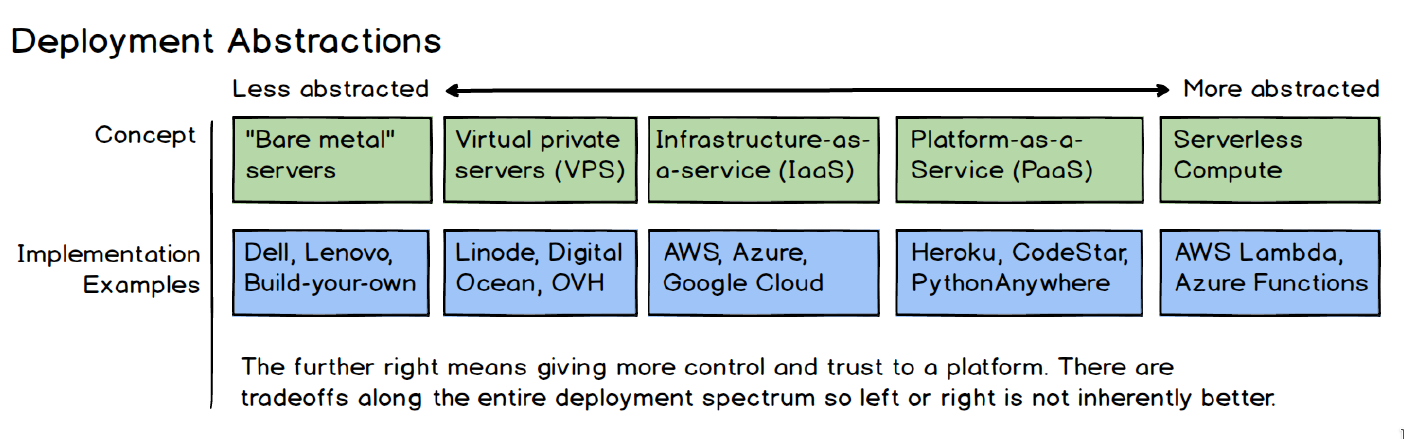
\includegraphics[width=\linewidth]{deploymentabstractions.png}
    \caption{Deployment abstractions: More vs less abstraction}
    \label{fig:deploymentabstractions}
\end{figure}

\subsection{The four pillars of serverless}
\begin{itemize}
    \item No server managment
    \item Flexible Scaling
    \item High Availability
    \item Never Pay for Idle
\end{itemize}

\subsection{Serverless FaaS: AWS Lambda}
\begin{itemize}
    \item Triggered by an event
    \item typically invoked in a few ms (warm start)
    \item Cold start issue: code that hasn't been used for a while takes longer to start
\end{itemize}

\begin{figure}[H]
    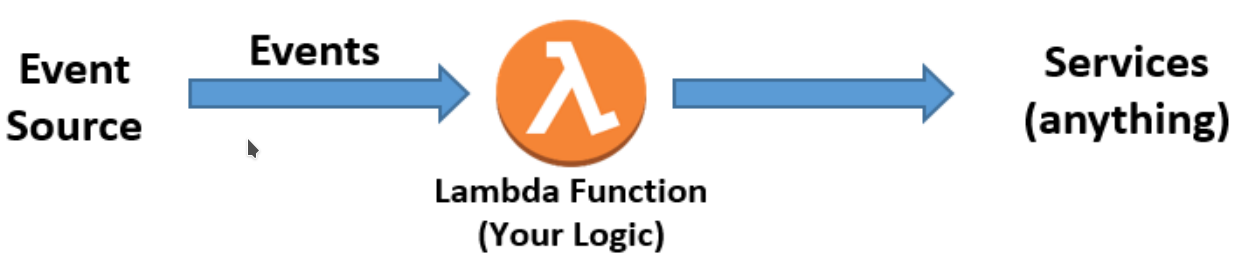
\includegraphics[width=\linewidth]{AWSLambdaTrigger.png}
    \caption{AWS Lambda: Event Triggers}
    \label{fig:awslambda}
\end{figure}

\subsection{The four stumbling blocks of serverless}
\begin{itemize}
    \item Performance Limitations
    \item Vendor Lock-in
    \item Monitoring and Debugging
    \item Security and Privacy
\end{itemize}

\subsection{Serverless usecases}
\begin{itemize}
    \item Event-driven data processing (resize uploaded images)
    \item Serverless webapplication (simple 3-tier app)
    \item Mobile  and IoT Apps (Airbnb smart home)
    \item Application Ecosystem (Alexa Skill)
    \item Event Workflow (image recognition and processing)
\end{itemize}

\section{L11: Scalable Systems}

\subsection{The Scale Cube}
\begin{figure}[H]
    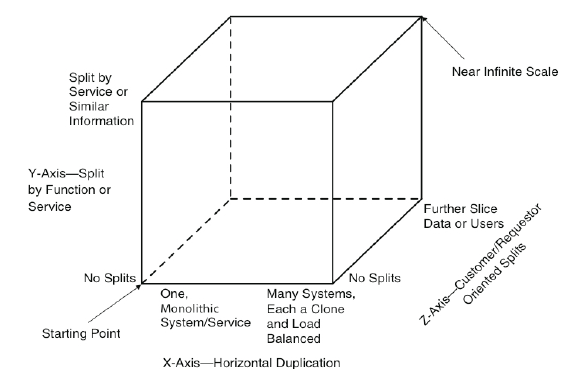
\includegraphics[width=\linewidth]{ScaleCube.png}
    \caption{The Scale Cube}
    \label{fig:scalecube}
\end{figure}

\begin{itemize}
    \item x-axis: \textbf{Horizontal Duplication}, unbiased cloning of services and data
    \item y-axis: \textbf{split by function or service}:refers to isolation (making different services)
    \item z-axis: \textbf{partitioning the domain of incoming requests}:data-partitioning, split relevant to 
    client (example: All customers from A-F are together processed, all customers from G-M, etc)
\end{itemize}

\subsection{Software architectures}
\begin{itemize}
    \item set of structures needed to reason about the system
    \item might be implicit
\end{itemize}

\subsection{Architectural Components and Patterns for scalable systems}
\begin{itemize}
    \item \textbf{Decoupled Components}: allows independent scalability of components; mechanisms to decouple:
    \begin{itemize}
        \item load balancers
        \item message queues
        \item message topics
        \item service registry
    \end{itemize}
    \item \textbf{Load Balancers}: distributing requests, hiding the server from client access, manage availability (HA),session affinity/sticky sessions
    \item \textbf{Session affinity/sticky sessions}:cookies managed by load balancer(duration based), cookies managed by application cookie
    \item \textbf{LB Algorithms}:(Weighted) Round Robin, Least connections
    \item \textbf{Message Topics}:messages are immeditaley pushed to subscribers, decouple producers and subscribers, concurrent processing
    \item \textbf{Message Queues}: Asynchronous: queue it now but run it later; seperates application logic; introduces latency
    \item \textbf{Service Registries}: resolve addresses for names, Leader voting (\textit{Byzantine Generel})
    \item \textbf{Automation}: autoscaler as sclaing can not be done manually (Metrics are CPU, RAM, Memory)
    \item Architectural Patterns: Service oriented architectures;  APIs are cloud requirement
\end{itemize}

\section{L13: MapReduce \& GFS/HDFS}

\begin{figure}[H]
    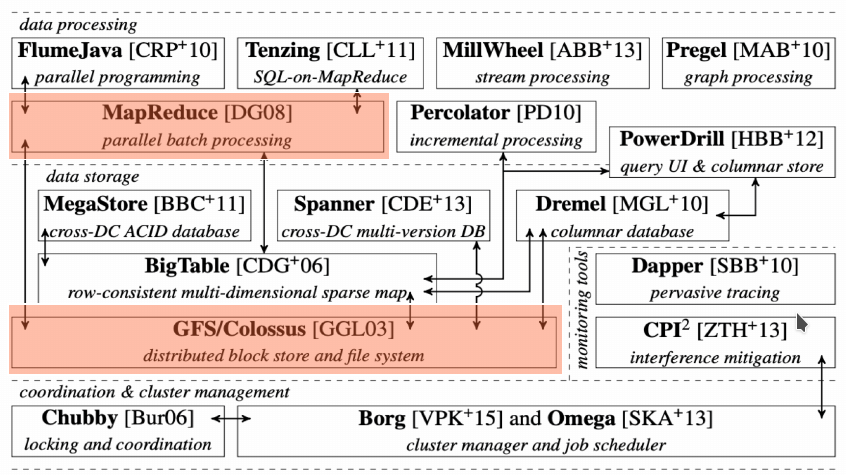
\includegraphics[width=\linewidth]{GoogleTechnologyStack.png}
    \caption{The Google Technology Stack}
    \label{fig:googlestack}
\end{figure}

\subsection{MapReduce: Basics}
\begin{figure}[H]
    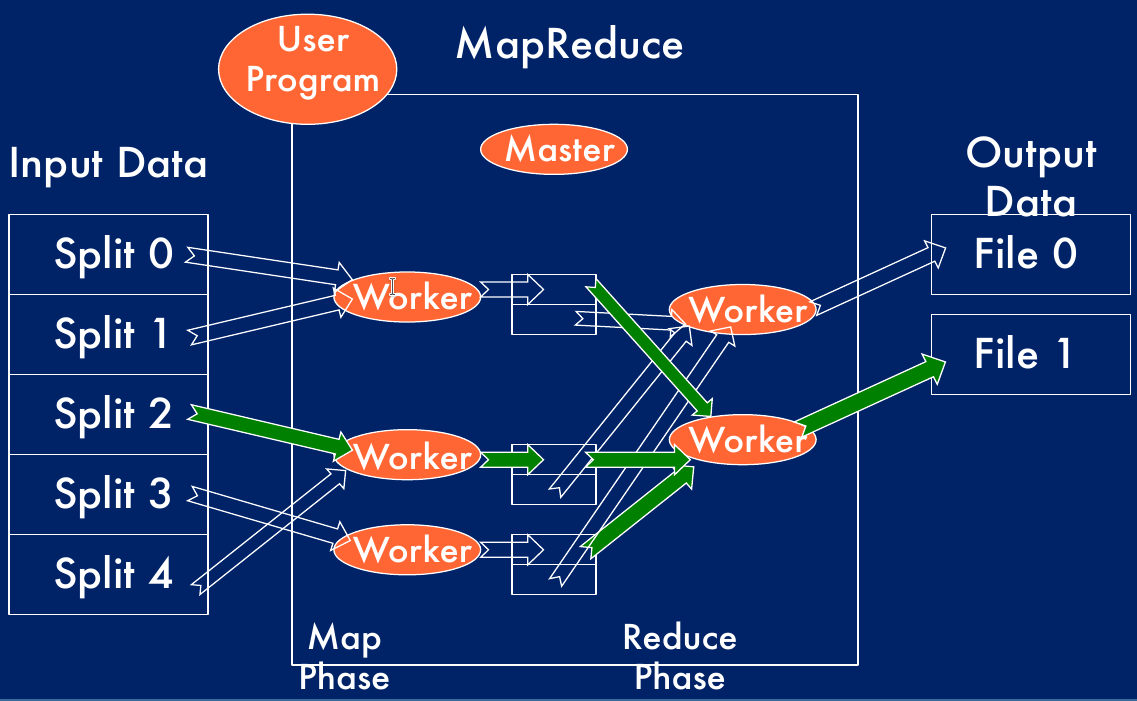
\includegraphics[width=\linewidth]{MapReduce.png}
    \caption{The MapReduce Technology}
    \label{fig:mapreduce}
\end{figure}

\begin{itemize}
    \item we have some input data
    \item \textit{Map phase}: master process assigns worker processes their part of the data, the data is than processed 
    \item \textit{Reduce phase}: other worker processes collect the processed data and reduce them
\end{itemize}

As the master pings the worker and a failure would be noticed really fast. This can now be handled by assigning other processes the task 
of the failed process.

\subsection{GFS - Google File System}
\begin{itemize}
    \item \textit{huge} scalable distributed storage using \textit{cheap} components
    \item files are divided in $64$ Mb blocks called \textbf{chunks} with a unique ID each (called \textbf{chunk handle})
    \item chunks are stored in \textbf{chunk servers}
    \item FT achieved through replication across multiple servers
    \item \textit{Write-control for replicas}: each change is performed on all replicas,synchronized via \textbf{leases} (\textbf{lease holder} is the \textbf{primary replica})
\end{itemize}

\begin{figure}[H]
    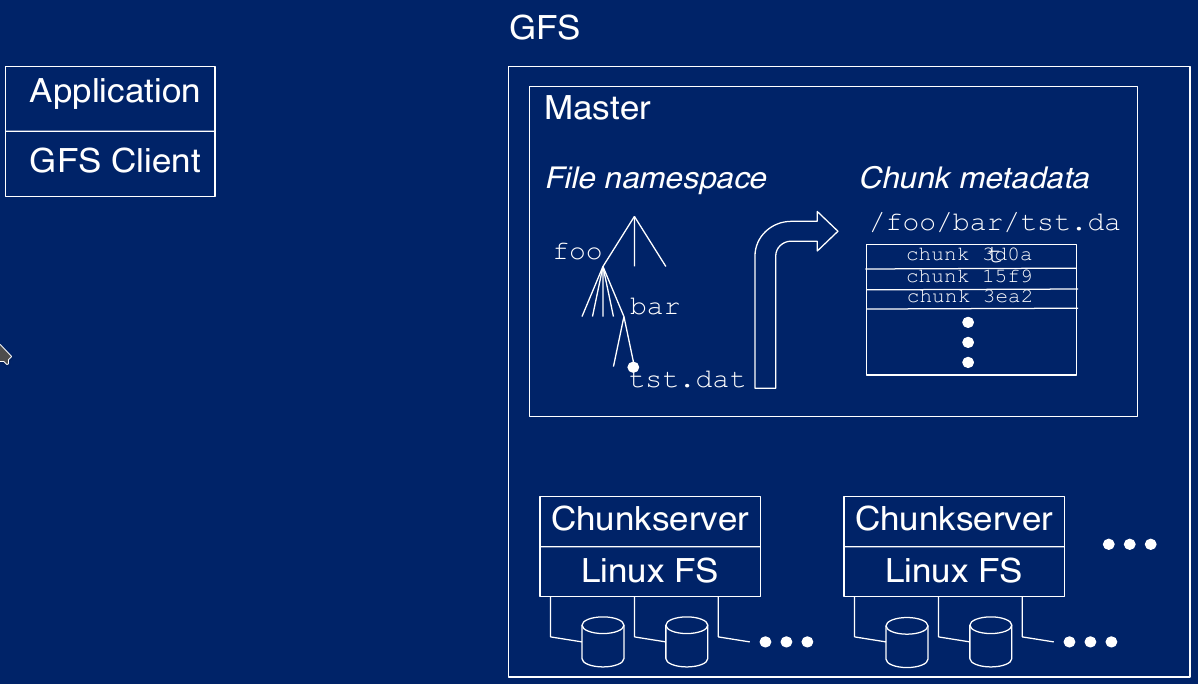
\includegraphics[width=\linewidth]{GFSArchitecture.png}
    \caption{The GFS Architecture}
    \label{fig:gfs}
\end{figure}

\subsection{HDFS - Hadoop File System}
\begin{itemize}
    \item \textit{HDFS}: same architecture as GFS with slightly different names
    \item \textit{HDFS 2.0}: new features: \textbf{NameNode HA}, \textbf{Snapshots}, \textbf{Federation} (horizontal scaling of NameNodes)
    \item \textit{HDFS 3.0}: currently beta status, major investement in \textbf{Erasure coding} (FT with more effiency,etc)
\end{itemize}

\section{L14: CAP, Paxos, BGP}

\subsection{CAP Theorem}
A good cloud might seek to achieve these three things, but it is only able to select two of them.
And as partition tolerance is mandatory for cloud applications we can only choose one of the other two.

\begin{itemize}
    \item \textbf{C}onsistency
    \item \textbf{A}vailability
    \item \textbf{P}artition Tolerance
\end{itemize}

\subsection{Paxos Approach}
\begin{itemize}
    \item \textbf{Paxos} is an approach to ensuring agreement of a series of asynchronous operations in distributed systems.
    \item achieve consensus, and ensure agreed actions can not be forgotten anymore
    \item dspite system messages being duplicate, lost, etc
    \item Paxos assumes messages are not deliberately malicious (BGP does)
\end{itemize}

\subsubsection{Three paxos rules}
\begin{itemize}
    \item Proposers: learn already accepted values
    \item Acceptors: let proposers know already accepted values, accept or reject proposals, reach consensus on chosing a particular proposal/value
    \item Learners: become aware of the chosen proposal/value and action it
\end{itemize}

\subsection{Types of Consistency}
\begin{itemize}
    \item \textbf{Strong Consistency}: after an update completes, every access will return the same updated value
    \item \textbf{Weak Consistency}: after an update completes, accesses are not guaranteed to return the updated value
    \item \textbf{Eventual Consistency}: eventually all access return the updated value (e.g. updates propagate in a lazy fashion)
\end{itemize}

\subsection{Byzantine Generals Problem}
\subsubsection{Byzantine Faults}
\begin{itemize}
    \item \textbf{Byzantine Fault}: different symptoms to different observers
    \item \textbf{Byzantine Failure}: loss of a system service due to Byzantine Fault
\end{itemize}

\subsubsection{Theoretical Problem}
\begin{itemize}
    \item there are a number of generals, each of them with one vote
    \item some of the generals are traitors and try to foil the other ones, by sending different votes to different generals (instead of the same vote to different generals)
    \item Key results of BG paper: BG can achieve consensus when $n\geq3m+1$ with $n$ loyal generals and $m$ traitors; To do so they must engange in $m+1$ rounds of message passing
    \item \textbf{Oral Message algorithm}: solves the problem but preventing BFs is very expensive in term of more bandwith and redundancy
\end{itemize}

\section{L15: The Hadoop Ecosystem}

\subsection{Important Components}
\begin{itemize}
    \item \textbf{Pig}: platform for batchmode analysis and large datasets, \textit{Pig Latin} is compiled to use MapReduce
    \item \textbf{Hive}: datawarehouse-software, allows big queries over distributed storage via SQL
    \item \textbf{YARN}: cluster resource managment and job scheduling, middleware layer between HDFS and various application listed here
    \item \textbf{Mahout}: scalable MachineLearning platform, runs on Hadoop/Spark
    \item \textbf{Hoyal/HBase}: HBase is non-relational distributed database (NoSQL), similar to \textit{Google BigTable}
    \item \textbf{Storm}: a distributed real-time stream-processing system
    \item \textbf{Giraph}: graph database, running MapReduce to process graphs
    \item \textbf{Spark}: analytics engine/framework for largescale dataprocessing that runs on YARN
\end{itemize}

\subsection{Hadoop Versions}
\begin{figure}[H]
    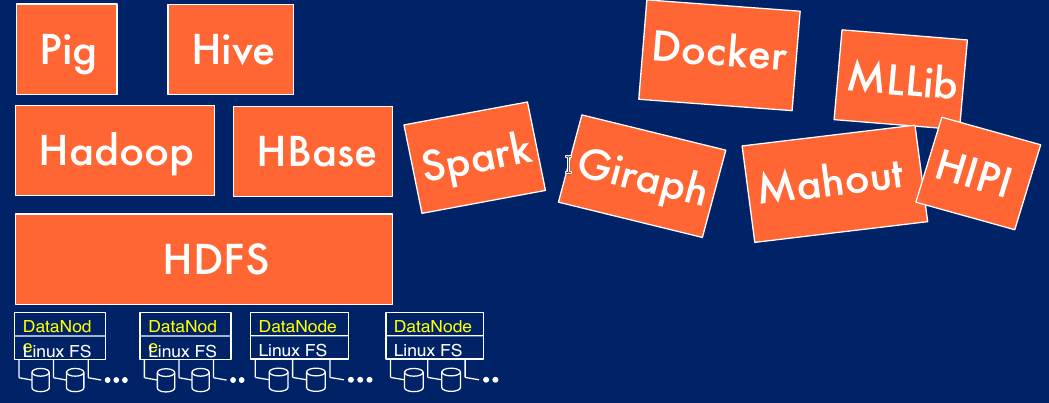
\includegraphics[width=\linewidth]{HadoopV1.png}
    \caption{The architecture of Hadoop 1.0}
    \label{fig:hadoopv1}
\end{figure}

\begin{figure}[H]
    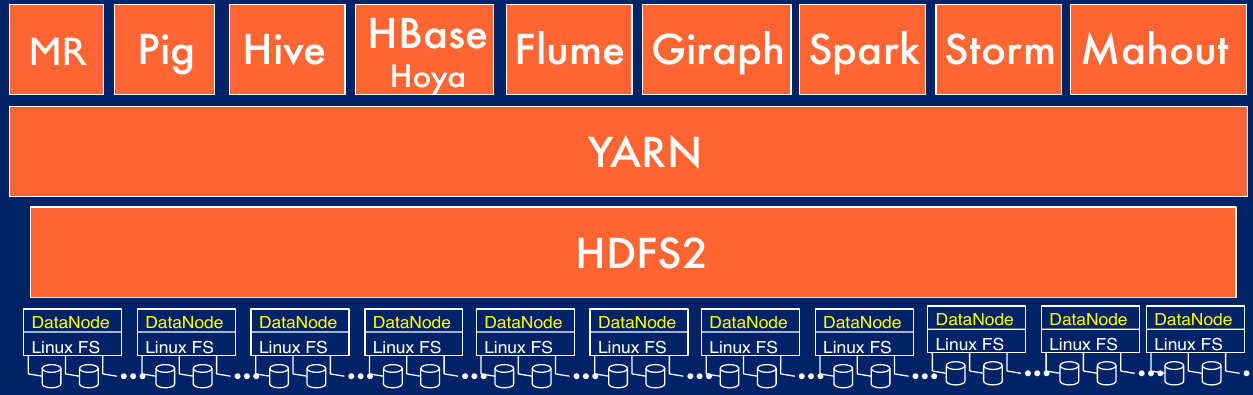
\includegraphics[width=\linewidth]{HadoopV2.png}
    \caption{The architecture of Hadoop 2.0}
    \label{fig:hadoopv2}
\end{figure}

\subsection{Hive}
TODO

\subsection{Pig}
TODO

\section{L16: Spark and In-Memory Methods}

\subsection{}
\begin{itemize}
    \item 
\end{itemize}

\section{L17: NoSQL Databases}

\subsection{Main classes of NoSQL databases}
\begin{itemize}
    \item \textbf{KeyValue DBs}: e.g. DynamoDB, Redis
    \item \textbf{Document DBs}: e.g. CouchDB, MongoDB
    \item \textbf{Column-Family DBs}: e.g. Cassandra, HBase
    \item \textbf{Graph DBs}: e.g. Giraph
\end{itemize}

\subsection{ACID \& CRUD}
\begin{itemize}
    \item \textbf{ACID}: oftered by RDBMSs, \textbf{A}tomacity \textbf{C}onsistency \textbf{I}solation \textbf{D}urablility
    \item \textbf{CRUD}: often CRUD is enough, \textbf{C}reate, \textbf{R}ead, \textbf{U}pdate, \textbf{D}elete
\end{itemize}
If you only want CRUD and do not care about the lack of ACID, you can choose NoSQL DBs instead of RDBMSs (which where engineered to run on a single server, which is hard to scale)

\subsection{KeyValue DBs}
\begin{itemize}
    \item very simple, schemaless
    \item often very fast
    \item DBs have different constraints (ACID, object limit size, etc)
\end{itemize}

\begin{figure}[H]
    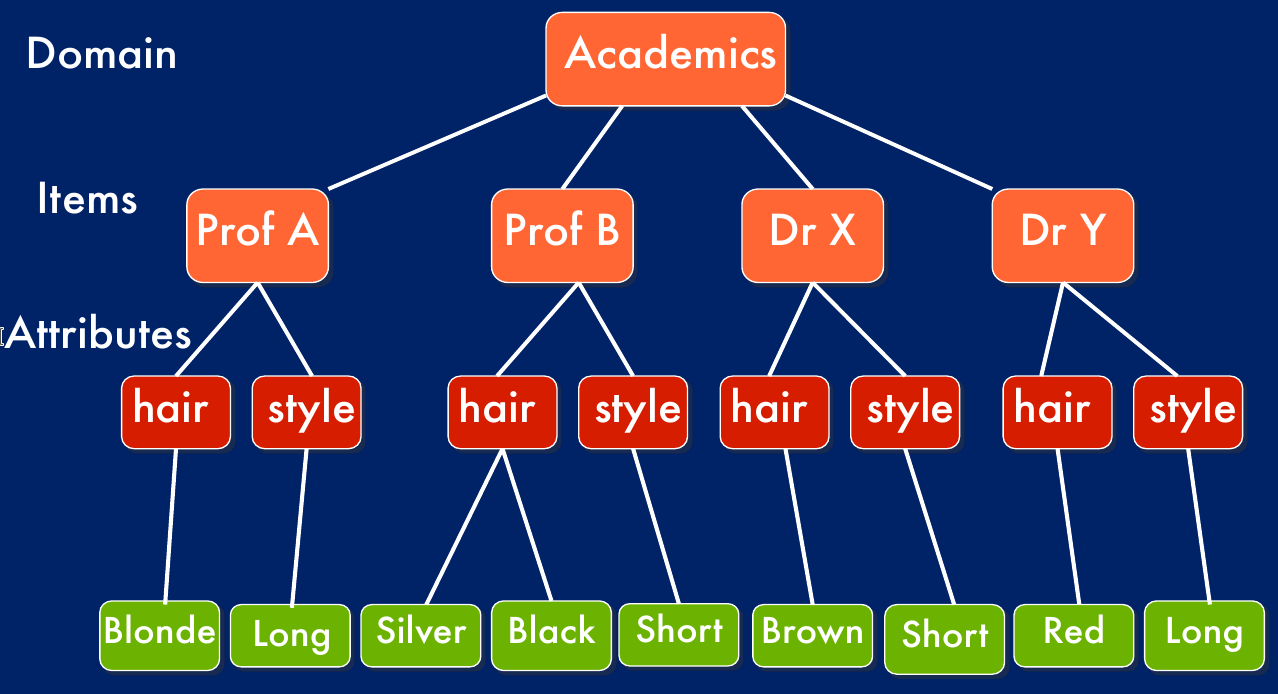
\includegraphics[width=\linewidth]{AmazonSimpleDB.png}
    \caption{Example of a KeyValue DB: Amazon Simple DB}
    \label{fig:amazonsimpledb}
\end{figure}

\subsection{Document DBs}
\begin{itemize}
    \item manage more complex data structures than KV datastores
    \item do not require you to define common structure for all datasets (like KV stores)
    \item a \textit{document} is a structured object, most commonly used are \textit{XML} and \textit{JSON}
\end{itemize}

\subsection{Column-Family DBs \& Columnar DBs}
\begin{itemize}
    \item for \textit{big data}, so \textit{VLDB} (Very Large Database)
    \item frequently used columns can be grouped together
    \item \textit{families} are like relational tables, inividual columns are more like key-value pairs
\end{itemize}

\subsection{Choices}
\begin{itemize}
    \item \textbf{Relational}: 
        \begin{itemize}
            \item \textit{good for}: when layout of data is known in before, but exact queries are not
            \item \textit{less good for}: when data is highly variable or deeply hierarchical
        \end{itemize}
    \item \textbf{Key Value}: 
        \begin{itemize}
            \item \textit{good for}: data largely independant, horizontal scaling, CRUD
            \item \textit{less good for}: perform non trivial queries
        \end{itemize}
    \item \textbf{Document}: 
        \begin{itemize}
            \item \textit{good for}: highly variable data, storing redundant data is not a problem
            \item \textit{less good for}: when data needs to be normalized
        \end{itemize}
    \item \textbf{Column-family}: 
        \begin{itemize}
            \item \textit{good for}: Big Data, data compression, have an idea how the queries will look like
            \item \textit{less good for}: when you don't know how data will be quiered
        \end{itemize}
    \item \textbf{Graph}: 
        \begin{itemize}
            \item \textit{good for}: applications with \textit{networks of relationships}
            \item \textit{less good for}: large scale situations where partitioning across nodes is necessary
        \end{itemize}
\end{itemize}
$\Rightarrow$ \textit{polyglot persistence model}: Use more databases, each playing a different role

\section{L18: Graph Databases}

\subsection{Network Basics}
\begin{itemize}
    \item a network/\textbf{Graph} consists of nodes/points/\textbf{Vertices}, which are connected with lines/\textbf{Edges} 
    \item \textbf{edges} are \textit{directed or undirected}, may be \textit{self-connections}, may be \textit{weighted}, may be \textit{multi-edges or hyper-edges}
    \item a \textbf{clicque} is a subgraph that is complete
    \item a \textbf{path} is a sequence of edges connecting two or more vertices, a \textbf{cycle} is a closed path
    \item node's \textit{indegree} counts ways to arrive it
    \item node's \textit{outdegree} counts ways to leave
    \item on a directed graph indegree and outdegree may differ
    \item Representing Graphs:
        \begin{itemize}
            \item \textit{Adjacancy List}
            \item \textit{Adjacancy Matrices}: the power of the matrix indicates the lenght of the path
        \end{itemize}
\end{itemize}

\subsection{PageRank}
\begin{itemize}
    \item PageRank for ranking webpage, where often linked pages are higher ranked
    \item \textit{Transition Matrix}: indicates the weight of each outgoing link/ edge (each page has $100\%$ for all his links together) 
    \item \textit{Dangling nodes problem}: A node with no outgoing edges simply jumps to a random site
    \item \textit{Damping}: off-network transitions appear now not with $0$ but with $\epsilon$ (very small) probability, (there is a dumping factor to specify this)
\end{itemize}

\subsection{Graph-processing}
\subsubsection{Pregel}
\begin{itemize}
    \item \textbf{Pregel} is a Google framework for network analysis
    \item it provides high scalability, fault-tolerance, flexibility in expressing arbitrary graph algorithms
    \item operates over a directed graph
\end{itemize}

\subsubsection{Apache Giraph}
\begin{itemize}
    \item open source equivalent of \textit{Pregel}
    \item integration in Hadoop ecosystem, efficiently loading data from HBase
\end{itemize}

\subsubsection{Bulk Sychronous Parallel Model}

\begin{figure}[H]
    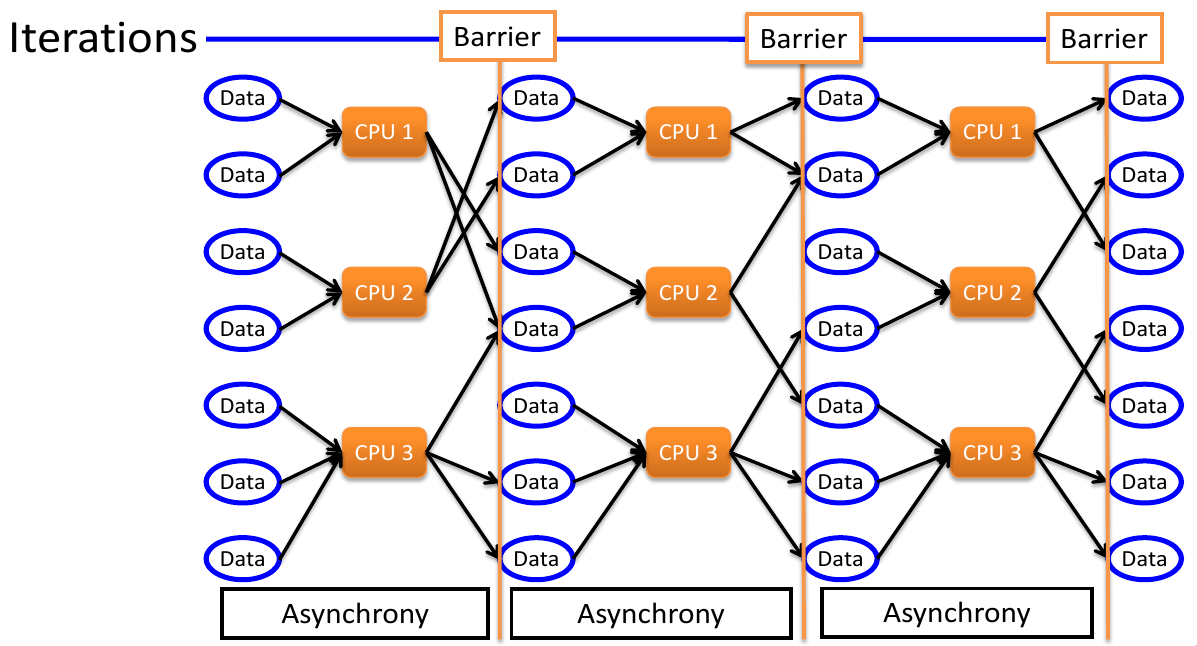
\includegraphics[width=\linewidth]{BSPModel.png}
    \caption{Bulk Synchronous Parallel Model}
    \label{fig:bspmodel}
\end{figure}

\begin{itemize}
    \item 3 steps:
        \begin{itemize}
            \item \textit{Concurrent Computation}: computation exclusively local to each node
            \item \textit{Communication}: messaging between nodes
            \item \textit{Barrier synchronisation}: checkpoints, block globally nodes before processing signalling received in a \textit{Superstep}
        \end{itemize}
    \item a sequence of \textit{supersteps} are run analogous to MapReduce
    \item during a superstep nodes can send messages, receive message sent in the last superstep, the function can modify the edges/state of verteces
    \item \textit{Algorithm Termination}: initinally every node is active, after finishing computation a node sets his state to inactive (until it receives a message and
    becomes active again), the algorithm terminates when all nodes are simultaneously inactive and there is no message in transit
    \item can be run distributed, then there is a master copy of the program managing/advicing all worker copies 
    \item fault tolerance: if a worker fails the master reassigns its vertices to another worker and restart the last superstep 
\end{itemize}

\section{L19: NewSQL $\&$ Event Stream Processing}

\subsection{NewSQL properties}
\begin{itemize}
    \item flexibility and scalability of NoSQL, support for SQL and/or ACID as RDBMS
    \item SQL as the primary interface
    \item ACID support for transactions
    \item Nonlocking concurrency controll
    \item high per node performance 
    \item parallel shared nothing architecture
    \item an example for this might be \textit{Google Spanner}
\end{itemize}

\subsection{Google Spanner}
\begin{itemize}
    \item lockfree distributed read-only transactions
    \item external consistency (ACID transactions)
    \item SQL queries
    \item officially AP (in terms of CAP)
    \item scales horizontally
    \item Spaner Zone Server Organisation:
        \begin{itemize}
            \item \textit{Zonemaster} assigns data to \textit{span servers}, 1 per zone
            \item \textit{Span server} serves data to clients, 300 - 1000 per zone
            \item \textit{Location proxies} are used by clients to locate span servers with correct data
            \item \textit{Universe master} has a status console, 1 per universe
            \item Zone Software Stack is part of \Cref{fig:zonesoftwarestack}
        \end{itemize}
    \item Spaner Application Model: supports unlimited tables in database within the universe, data actually stored on 3 replicas
    \item Open Source DBs based on Spanner: \textit{CockroachDB}, \textit{YugaByte}
\end{itemize}

\begin{figure}[H]
    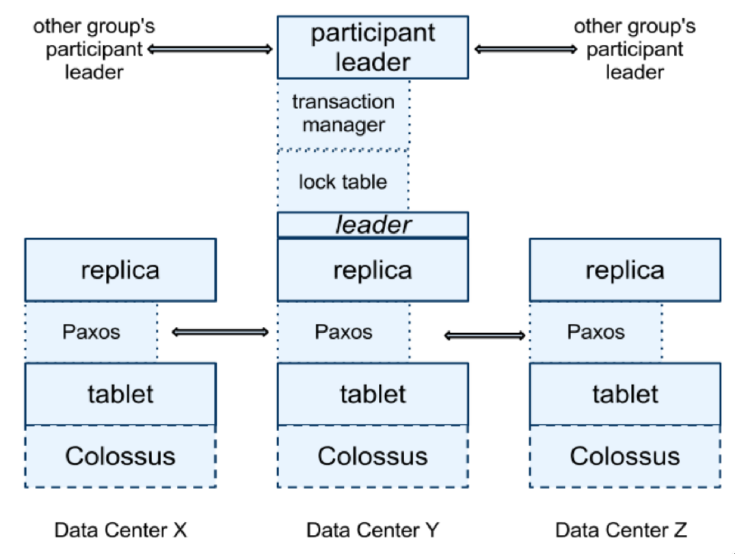
\includegraphics[width=\linewidth]{ZoneSoftwareStack.png}
    \label{fig:zonesoftwarestack}
\end{figure}

\subsubsection{Google TrueTime}
\begin{itemize}
    \item used in and makes \textbf{Google Spanner} possible
    \item every Google datacentre has an atomic clock
    \item clients poll TimeMasters (GPS and atomic clocks)
    \item TrueTime API is Google proprietary
\end{itemize}

\subsubsection{Google F1 Database}
\begin{itemize}
    \item database built on top of Spanner
    \item five replicas needed for HA
    \item Geography: replicas spread around the world to survive regional disasters
    \item High Throughput, but different approaches have to be done to deal with high latency
    \item One System for \textit{OLAP} and \textit{OLTP} (=\textit{HTAP})
\end{itemize}

\subsection{Real Time Event Streaming}
\begin{itemize}
    \item different use cases (e.g. network and Infrastructure monitoring, sensor data, commerce and retail marketing)
    \item Requirements: data arrives in real time (online), High throughput, low latency, FT
\end{itemize}

\subsubsection{Systems for RTSP}
\begin{itemize}
    \item General Architecture: Components(Source, Processing, Sinks), Framework provides message queueing, ressoure manager to allocate nodes tasks
\end{itemize}

\subsubsection{Apache Storm}
\begin{itemize}
    \item pioneer in realtime processing
    \item works on unbounded stream of messages 
    \item appropriate for low latency
    \item \textit{Storm provides the transformation of streams, so to transform one stream into another one.}
    \item topology runs forever or until it gets killed. No data loss is guaranteed even in the case of machine failures or messages get dropped
    \item Problems for Storm: no exactly once-guarantees, consistency, difficult to combine batch and stream processing, straggler tolerance
\end{itemize}

\subsubsection{Discetrized Streams and Spark Streaming}
\begin{itemize}
    \item \textit{Buffer and Compute} pattern
    \item near real time
    \item avoid overhead from Disk I/O that Hadoop faced 
\end{itemize}
TODO

\subsubsection{Apache Kafka}
\begin{itemize}
    \item TODO
\end{itemize}

\section{L20: Cloud Security}

\subsection{CSA Threacherous Twelve Threat List}
\begin{itemize}
    \item \textbf{Data Breachers}
    \item \textbf{Identity/Credential/Access managment}
    \item \textbf{Insecure interfaces and APIs}
    \item \textbf{System vulnerabilities}
    \item \textbf{Account hijacking}
    \item \textbf{Malicious insiders}
    \item \textbf{Abuse of cloud services}
    \item \textbf{Data loss}
    \item \textbf{Insufficient due diligence}
    \item \textbf{abuse \& nefarious use of cloud services}
    \item \textbf{Denial of Service}
    \item \textbf{Shared Technology Issues}
\end{itemize}

\subsection{Academic Cloud Research}
\begin{itemize}
    \item Five Pitfalls:
        \begin{itemize}
            \item Infrastructure at scale
            \item Abstraction
            \item Non-reproducible results
            \item Rebranding
            \item Industrial relations
        \end{itemize}
    \item Five Opportunitiers:
        \begin{itemize}
            \item User-driven Research
            \item Programming models
            \item Debugging large scale applications
            \item PaaS Environments
            \item Elasticity
        \end{itemize}
\end{itemize}

\section{L21: DevOp}

\subsection{Software Design Methods}

\begin{figure}[H]
    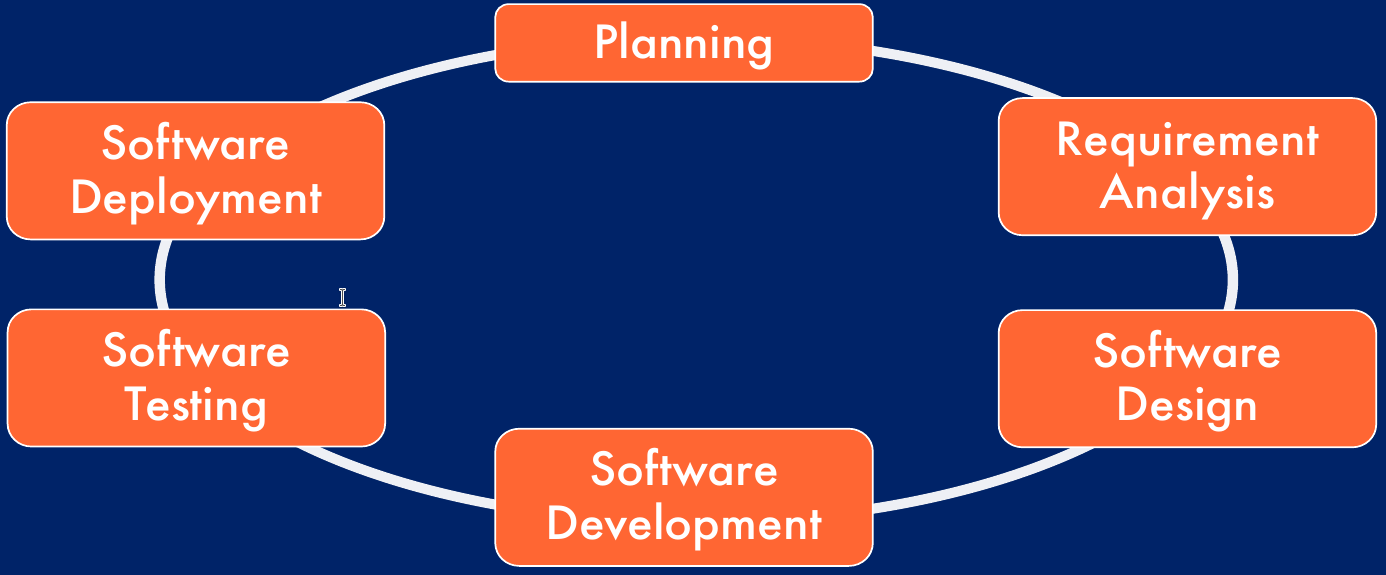
\includegraphics[width=\linewidth]{SDLC.png}
    \caption{Software Design Lifecycle SDLC}
    \label{fig:sdlc}
\end{figure}

\begin{figure}[H]
    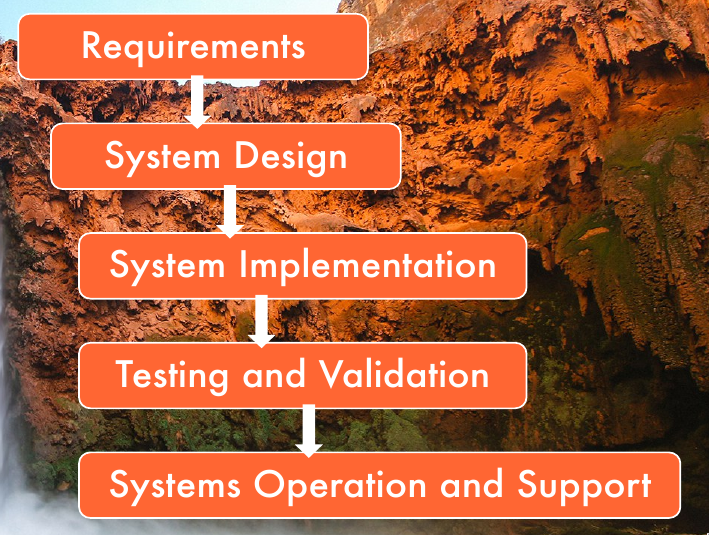
\includegraphics[width=\linewidth]{Waterfallmodel.png}
    \caption{Before Agile Dev: Waterfall model}
    \label{fig:waterfallmodel}
\end{figure}

\begin{itemize}
    \item Waterfall is inefficient in non-trivial projects
    \item $\Rightarrow$ Agile Developement Methods:
        \begin{itemize}
            \item Iterative developement cycles
            \item XP (extreme programming)
            \item Scrum, sprints are often 2 weeks long
        \end{itemize}
\end{itemize}

\subsection{DevOps Traits}
\begin{itemize}
    \item Goal: \textit{Releasing updates as quickly as possible without losing quality}
    \item Developers want \textit{agility}, Operations want \textit{stability}
    \item \textbf{Cross-functional Dev/Ops Teams}:
        \begin{itemize}
            \item \textit{Collaboration}: sprint dev teams may include QA from Ops
            \item \textit{Responsibility}: team is responsible for end-to-end quality product
            \item \textit{Awareness}: both learn potential issues from the other one
            \item \textit{Communication}: tools like Slack or Jira
        \end{itemize}
    \item \textbf{Frequent Code Commits and Builds}:
        \begin{itemize}
            \item \textit{Continuous Integration}
            \item \textit{Continuous Delivery}
            \item \textit{Continuous Deployment}
        \end{itemize}
    \item \textbf{Robust Product Releases}:
        \begin{itemize}
            \item \textit{Fail-fast philosophy}
            \item \textit{Integrated Monitoring}
            \item \textit{Integrated Security(SecOps)}
        \end{itemize}
    \item \textbf{Consistent Deployment Environments}:
        \begin{itemize}
            \item \textit{Identical Environments}
            \item \textit{Infrastructure as Code (IaC)}
        \end{itemize}
\end{itemize}

\begin{figure}[H]
    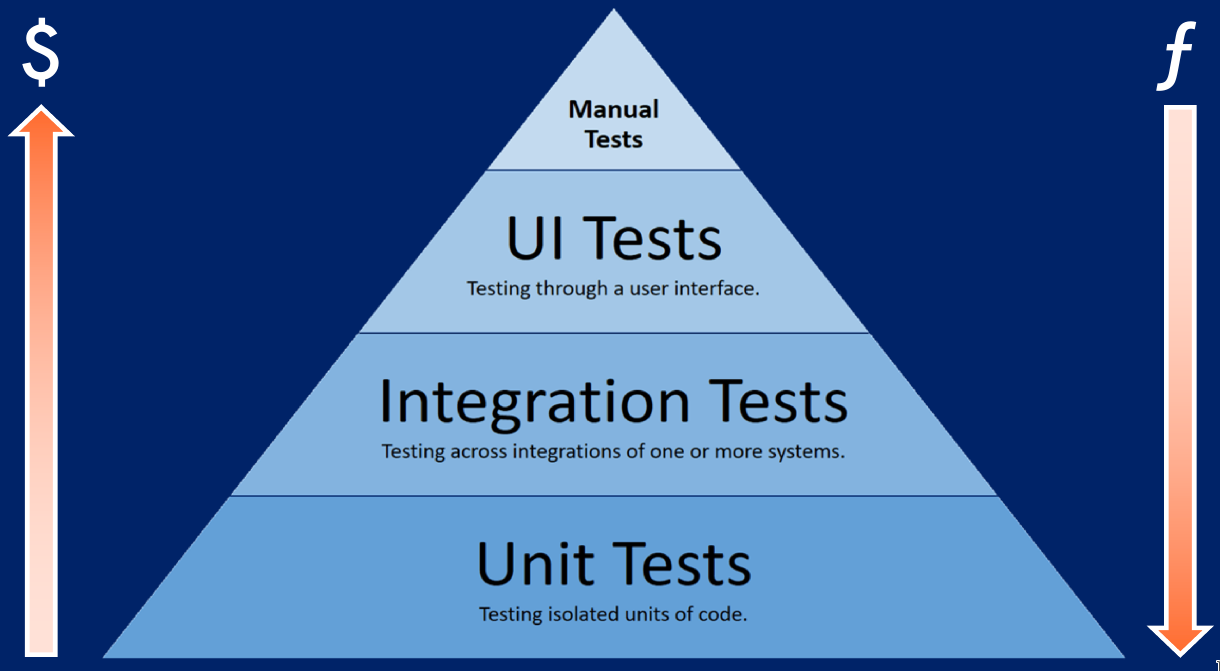
\includegraphics[width=\linewidth]{CostvsFreqTesting.png}
    \caption{Automated Tests: Costs vs Frequency}
    \label{fig:autotest}
\end{figure}

\subsection{Infrastructure as Code}
\begin{itemize}
    \item \textbf{Automate} the creation, deletion, updates to infrastructure
    \item \textbf{Consistent repeatability} for multiple environments
    \item \textbf{Version control} the infrastructure
    \item dependent on IaaS \textbf{APIs}
    \item typically implemented using \textit{Configuration managment}, \textit{Orchestration}, \textit{Scripting}
    \item most popular IaC templating engines: \textit{Terraform}, \textit{CloudFormation(AWS)}
    \item \textit{CloudFormation Template} Sections:
        \begin{itemize}
            \item \textit{Ressources}
            \item \textit{Parameters}
            \item \textit{Conditions}
            \item \textit{Mappings}
            \item \textit{Metadata}
            \item \textit{Transform}
            \item \textit{Outputs}
        \end{itemize} 
\end{itemize}



\section{Possible exam Questions}

\begin{figure}[H]
    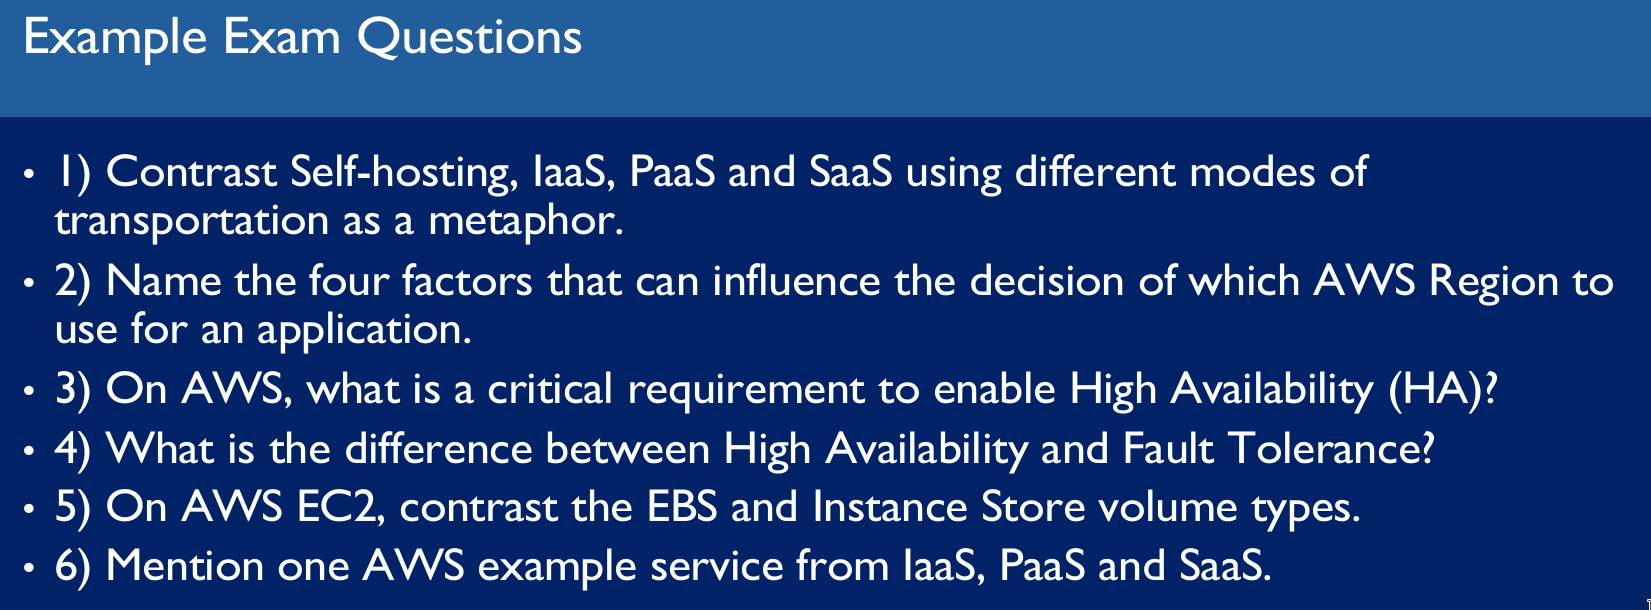
\includegraphics[width=\linewidth]{ExampleExamQuestions01.png}
    \label{fig:examquestion01}
\end{figure}

\begin{figure}[H]
    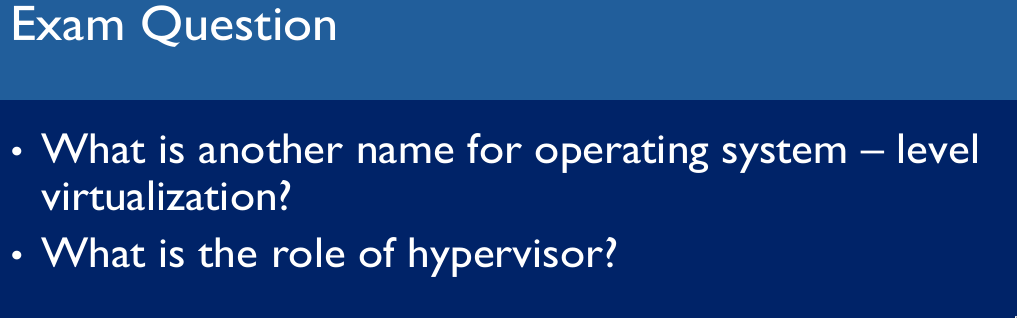
\includegraphics[width=\linewidth]{ExampleExamQuestions02.png}
    \label{fig:examquestion02}
\end{figure}

\begin{figure}[H]
    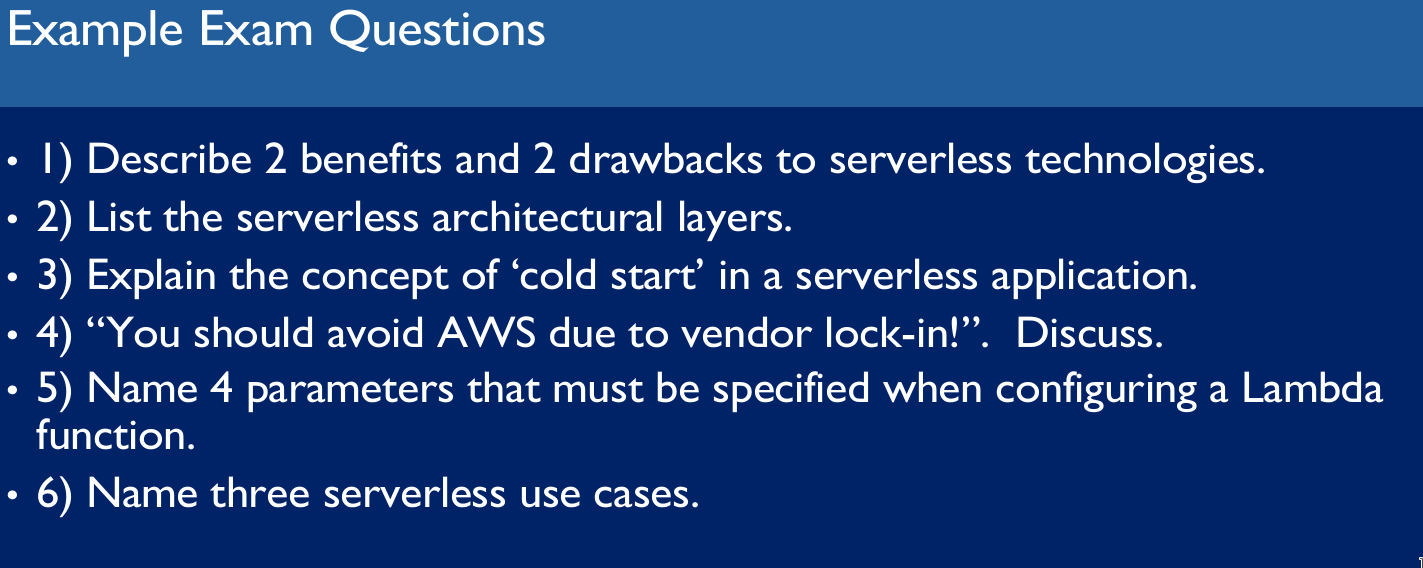
\includegraphics[width=\linewidth]{ExampleExamQuestions03.png}
    \label{fig:examquestion03}
\end{figure}

\begin{figure}[H]
    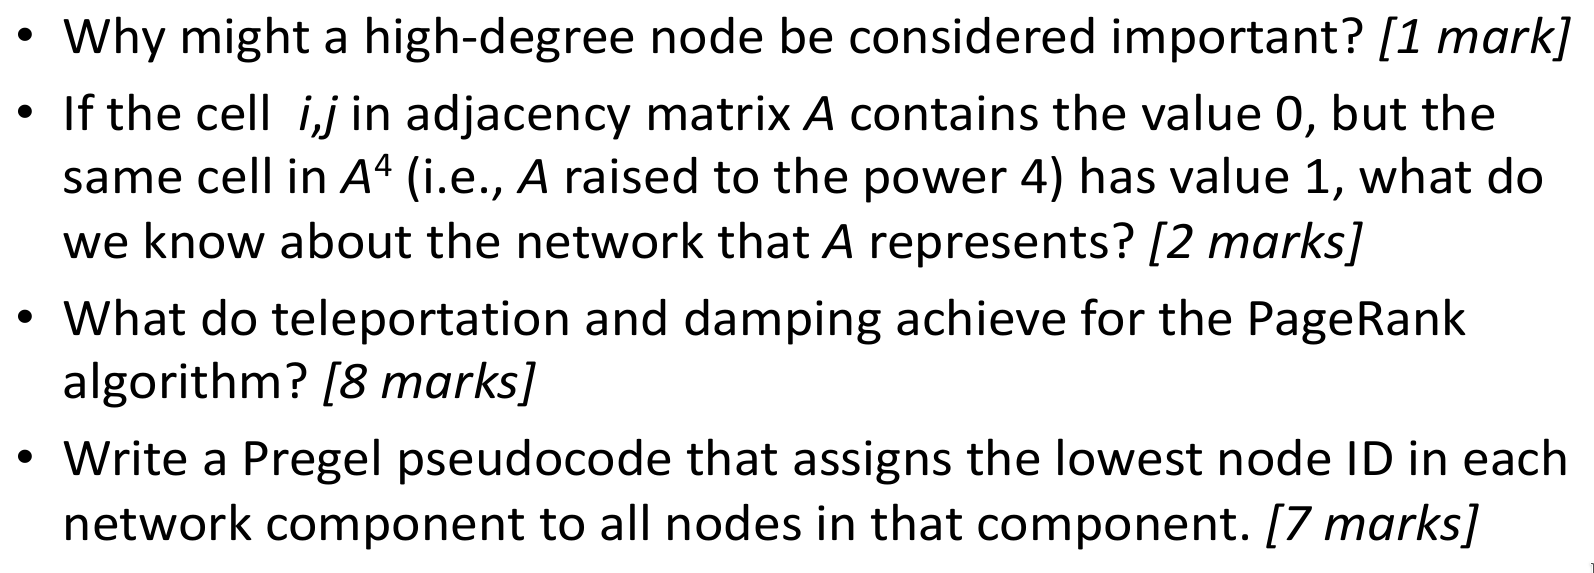
\includegraphics[width=\linewidth]{ExampleExamQuestions04.png}
    \label{fig:examquestion04}
\end{figure}

\begin{figure}[H]
    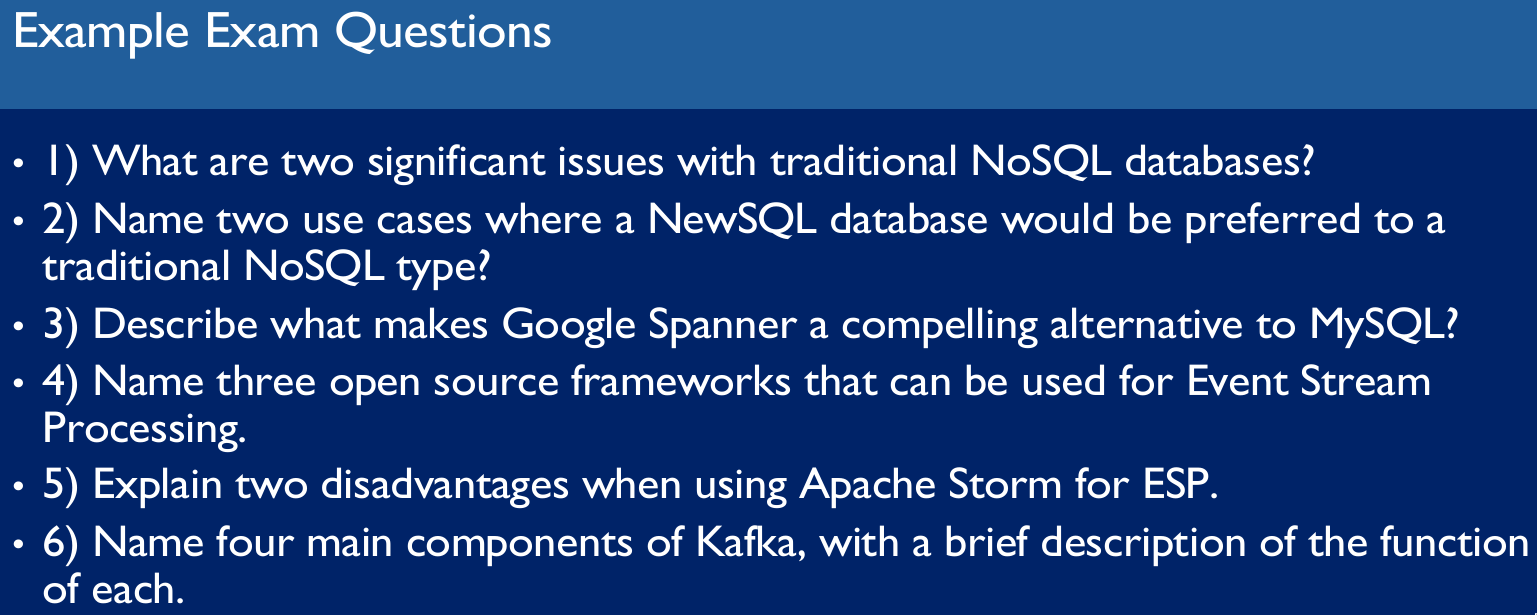
\includegraphics[width=\linewidth]{ExampleExamQuestions05.png}
    \label{fig:examquestion05}
\end{figure}

\begin{figure}[H]
    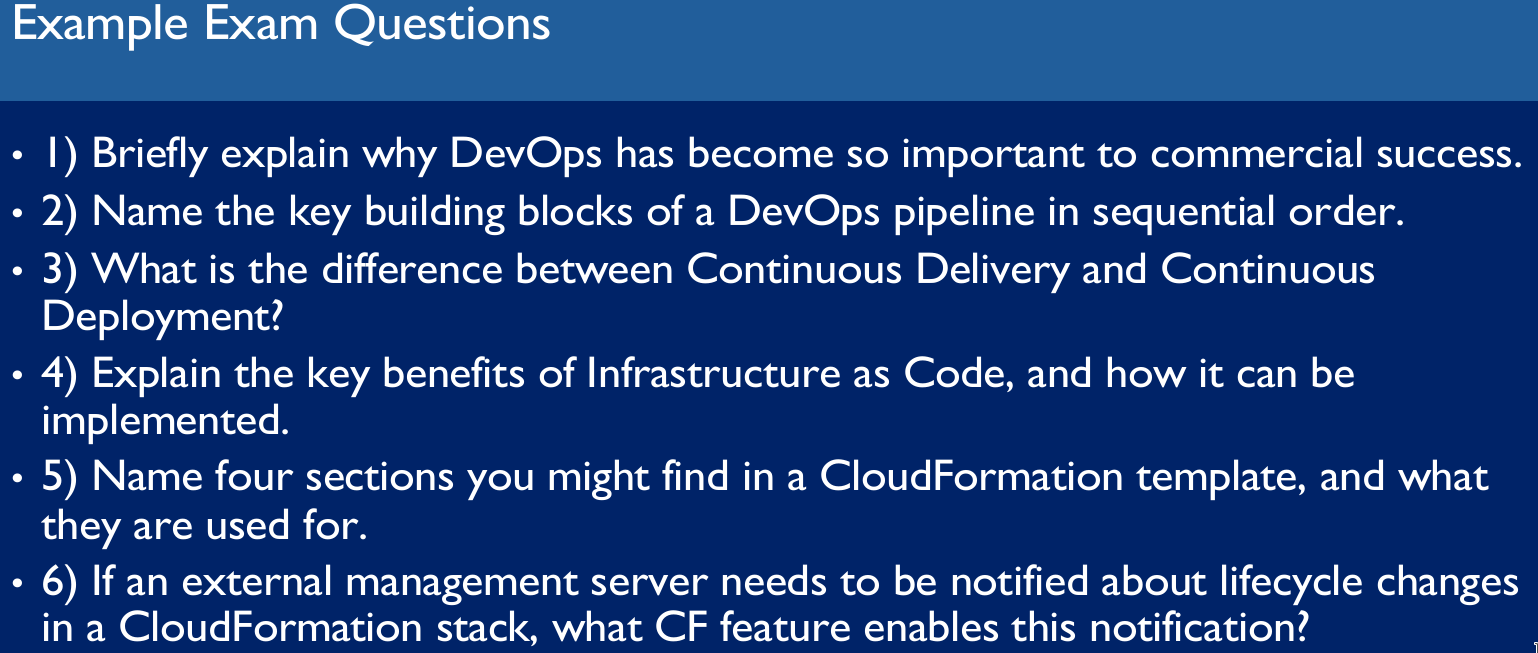
\includegraphics[width=\linewidth]{ExampleExamQuestions06.png}
    \label{fig:examquestion06}
\end{figure}

\vspace*{\fill}
    \pagebreak
\end{multicols}
\end{document} 
